\section{Détection d'obstacles}

Afin de détecter les obstacles, nous avons voulu réaliser un algorithme qui suit le protocole suivant :
\begin{enumerate}
    \item Récupération des mesures.
    \item Discrétisation angulaire.
    \item Détermination des groupes de points consécutifs sans valeurs au delà du seuil défini dans le fichier de configuration.
    \item Création d'un obstacle dont les attributs sont les points détectés selon l'étape précédente.
    \item Détermination d'un centre de l'objet à partir des points définissant l'obstacle.
    \begin{figure}[htp]
    \centering
    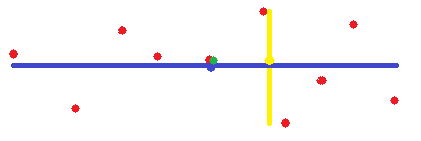
\includegraphics[width=8cm]{images/Detection/centre-object.png}
    \caption{Détermination du centre obstacle}
\end{figure}
\newline
Supposons que les points rouges correspondent à une liste de mesure que l'on a affecté à un obstacle. Le centre (vert) est alors défini en coordonnées polaire par l'angle médian (bleu) et la distance médiane (jaune).
\end{enumerate}

\subsection{Programmation en Python d'un affichage dynamique}
\tab Afin de visualiser les données extraites du LiDAR, nous avons réalisé un affichage dynamique. Cet affichage permet la visualisation des obstacles définis dans le protocole ci-dessus.
%compléter
Nous avons de plus décidé d’uniformiser les unités du code en effectuant une conversion complète des programmes en Radian.
Cela nous aura également donné l’occasion de faire un affichage ressemblant à celui d’un sonar.

\begin{figure}[htp]
    \centering
    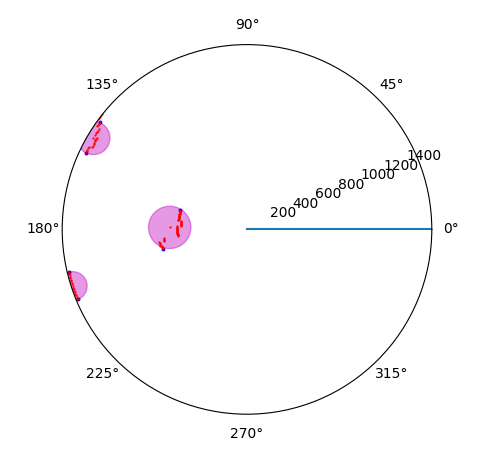
\includegraphics[width=10cm]{images/Detection/sans_piste_ni_kalman_polaire01.png}
    \caption{Affichage en coordonnées polaires.}
\end{figure}
\begin{figure}[htp]
    \centering
    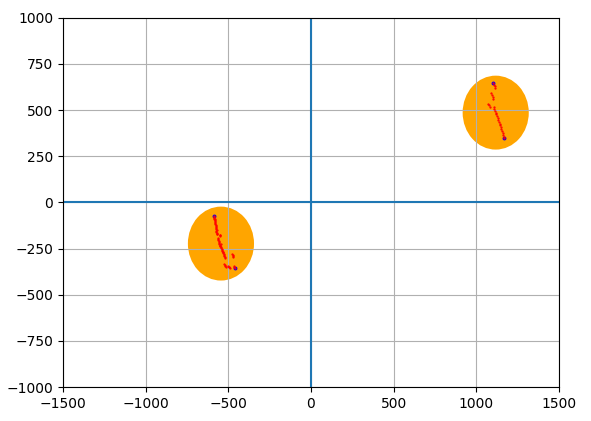
\includegraphics[width=10cm]{images/Detection/sans_piste_ni_kalman_cartesien01.png}
    \caption{Affichage en coordinnées cartesiennes.}
\end{figure}

%expliquer pourquoi on appelle ça "affichage polaire" et "affichage cartesien" ? -> Done

\newpage
\subsection{Amélioration des performances}
\tab Durant nos phases de tests, nous nous sommes rendu compte que l’élément bloquant n’était pas le traitement des données mais bel et bien l’acquisition. En effet, on s'est rendu compte que la prise de mesures sur plusieurs tours avant traitement nuisait de façon conséquente à la réactivité du système. On avait alors une rémanence des obstacles qui posait un vrai soucis.

\tab Nous avons donc décidé de paralléliser les tâches à l’aide de Threads Python pour acquérir des données en continu et de ne les récupérer que lorsque l’algorithme de traitement le demande. On a donc pu supprimer les obstacles rémanents qui nous posaient problème. Il semble en effet plus cohérent que ce soit le traitement des données qui conditionne la réactivité du système et non pas l'acquisition des données. 

\tab En définitive, le problème de l'acquisition des mesures pour la détection d'obstacle se fait de la façon la plus simple possible : on remplit progressivement une queue Python contenant les distances de chaque angle reçu, dans le sens anti-trigonométrique, chaque indice étant associé à un angle à 0.5 degré près. Le Thread principal, de traitement de données, récupère alors des éléments dans cette queue dès qu'il en a besoin. Au départ, l'idée était d'utiliser des sémaphores pour gérer l'accès à une liste, mais en utilisant des queues Python nous n'avons plus besoin de ces sémaphores explicites.

% Faire un cadre qui explique la notion de queue en Python

% Parler des threads en Python. Parler des problèmes rencontrés avec elles et les solutions proposées.

\tab Ainsi, même si on peut supposer que l'on perd en fiabilité dû au fait qu'on ne réalise plus une moyenne sur plusieurs valeurs ou bien que l'on acquiert pas nécessairement une valeur à chaque tour pour chaque angle, le gain en réactivité et la perte d'obstacles rémanents contrebalancent complètement cette perte. D'autant plus que cette perte de fiabilité, en supposant qu'elle existe, sera grandement corrigée par le traitement des obstacles, notamment avec le filtrage de Kalman.

%parler des sémaphores.  -> On s'en sert pas vraiment directement